\documentclass[12pt,letterpaper]{article}
\usepackage[latin1]{inputenc}
\usepackage[spanish]{babel}
\usepackage{amsmath}
\usepackage{amsfonts}
\usepackage{amssymb}
\usepackage{graphicx}
\usepackage[left=2cm,right=2cm,top=2cm,bottom=2cm]{geometry}
\title{\textbf{Robótica Industrial}\\ Simulación de un sistema PID en simulink }
\author{Sánchez Sandoval Carlos Alberto} 
\begin{document}
\maketitle

\begin{flushleft}
El controlador derivativo se opone a desviaciones de la se\~{n}al de entrada, con una respuesta que es proporcional a la rapidez con que se producen \'estas 
 siendo que:\\

\begin{center}
\textbf{$ k_{P}+k_{D}s $}\\ 
\end{center}

\begin{flushleft}
Como bien se sabe estamos sumando $k_{P}$ mas el derivador del sistema $ k_{D}s $\\
Se comienza cargando las librer\'ias de simulink para generar las condiciones y poder generar el PD 
\\
\end{flushleft}
\begin{center}
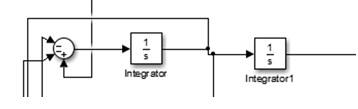
\includegraphics[scale=1]{simulink2.jpg}\\
\end{center}  
Colocamos un sumador y dos integradores al principio  que serán la base para crear nuestro PD \\
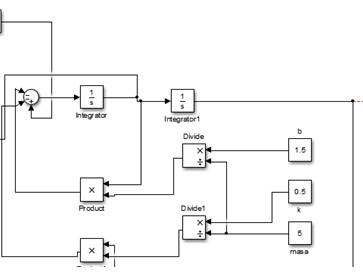
\includegraphics[scale=1]{simulink2-1.jpg}\\ 
\begin{flushleft}
Se agregan 3 constantes que ser\'an los valores que tendr\'an nuestras letras para el calculo del sistema. Las cuales estar\'an multiplicando y dividiendo en  cada divisor que en este caso se agregan dos.  
 
\end{flushleft}
\begin{flushleft}
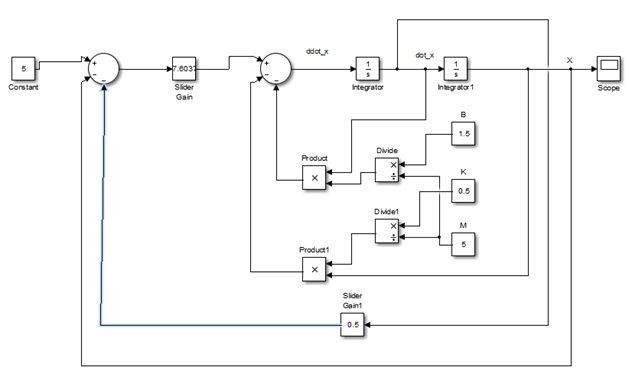
\includegraphics[scale=1]{simulink2-2.jpg}\\  
Entonces, el producto de cada uno de  los derivadores ser\'a multiplicado por el sumado y agregamos otra constante que estar\'a sumando el producto del primer integrador y le daremos valores de rangos que llevaran al primer sumado. \\
por lo tanto, cuando vemos la visualizaci\'on de la gr\'afica tendríamos un sistema subamortiguado en este caso  el sistema esta controlado a 5 que es el rango de la gr\'afica.\\
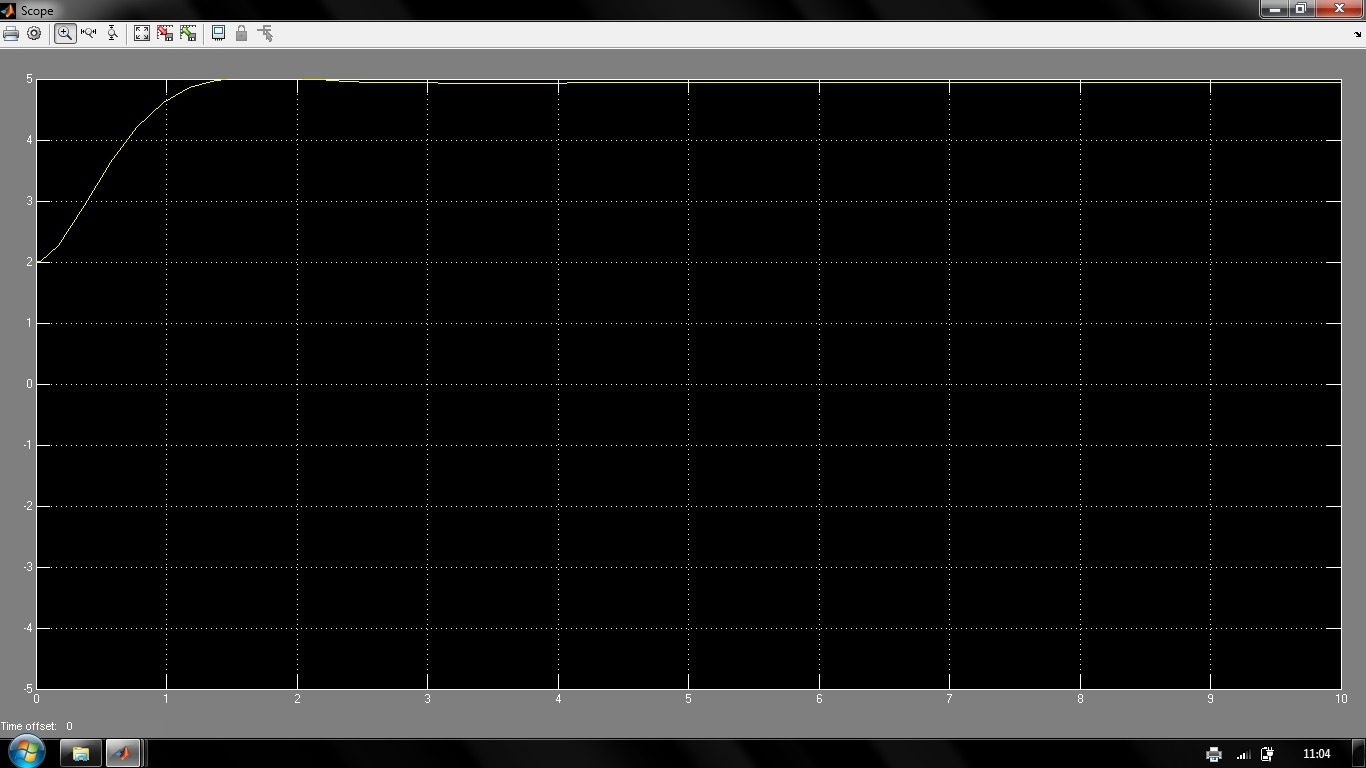
\includegraphics[scale=.5]{captura_simulink.jpg} 
  
\end{flushleft}
\end{flushleft} 
\textbf{Conclusi\'on: Como se pudo observar el utilizar la aplicaci\'on de simulink  para poder visualizar   un controlador PD  es muy efectivo ya que podemos realizar asta un PID para el control de un sistema   } 
\end{document}

